\chapter{Numerika}
\begin{figure}[!ht]
    \centering
    \resizebox{.6\textwidth}{!}{% This file was created with tikzplotlib v0.10.1.
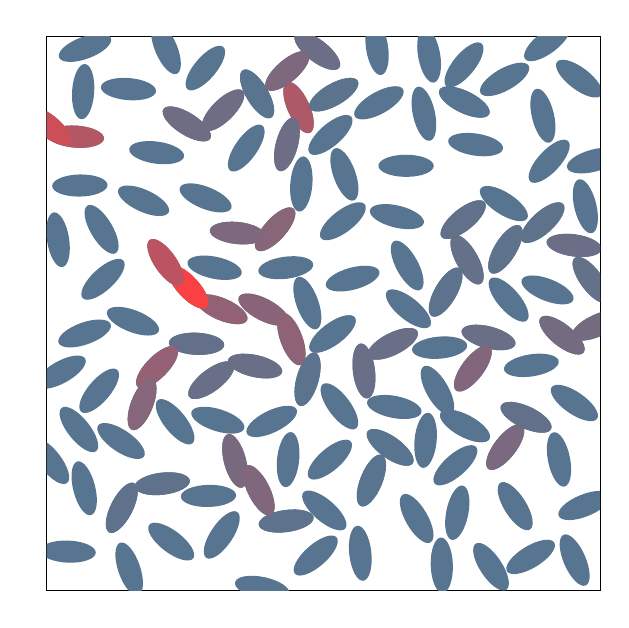
\begin{tikzpicture}

\definecolor{darkgray176}{RGB}{176,176,176}
\definecolor{gray116107129}{RGB}{116,107,129}
\definecolor{gray121105127}{RGB}{121,105,127}
\definecolor{gray122105127}{RGB}{122,105,127}
\definecolor{gray126104125}{RGB}{126,104,125}
\definecolor{gray129103124}{RGB}{129,103,124}
\definecolor{gray131102123}{RGB}{131,102,123}
\definecolor{gray133102122}{RGB}{133,102,122}
\definecolor{gray136101120}{RGB}{136,101,120}
\definecolor{gray137100120}{RGB}{137,100,120}
\definecolor{gray14398117}{RGB}{143,98,117}
\definecolor{gray14698116}{RGB}{146,98,116}
\definecolor{gray14797115}{RGB}{147,97,115}
\definecolor{indianred17389103}{RGB}{173,89,103}
\definecolor{indianred17987100}{RGB}{179,87,100}
\definecolor{indianred1878496}{RGB}{187,84,96}
\definecolor{indianred2047988}{RGB}{204,79,88}
\definecolor{slategray100112137}{RGB}{100,112,137}
\definecolor{slategray101112137}{RGB}{101,112,137}
\definecolor{slategray104111135}{RGB}{104,111,135}
\definecolor{slategray105111135}{RGB}{105,111,135}
\definecolor{slategray106110135}{RGB}{106,110,135}
\definecolor{slategray107110134}{RGB}{107,110,134}
\definecolor{slategray109109133}{RGB}{109,109,133}
\definecolor{slategray110109132}{RGB}{110,109,132}
\definecolor{slategray87117144}{RGB}{87,117,144}
\definecolor{slategray88116143}{RGB}{88,116,143}
\definecolor{slategray90115142}{RGB}{90,115,142}
\definecolor{slategray92115141}{RGB}{92,115,141}
\definecolor{slategray93114141}{RGB}{93,114,141}
\definecolor{slategray94114140}{RGB}{94,114,140}
\definecolor{slategray95114140}{RGB}{95,114,140}
\definecolor{slategray96113139}{RGB}{96,113,139}
\definecolor{slategray98113138}{RGB}{98,113,138}
\definecolor{slategray99112138}{RGB}{99,112,138}
\definecolor{tomato2496568}{RGB}{249,65,68}

\begin{axis}[
    x=2, y=2,
    x grid style={darkgray176},
    xmin=0, xmax=100,
    y grid style={darkgray176},
    ymin=0, ymax=100,
    tick style={draw=none},
    yticklabels={,,},
    xtick
]
\draw[draw=none,fill=slategray87117144,rotate around={40.875524397656:(axis cs:51.1648570437529,23.6259558337609)}] (axis cs:51.1648570437529,23.6259558337609) ellipse (5 and 2);
\draw[draw=none,fill=slategray87117144,rotate around={-66.4590190945365:(axis cs:95.3923133763875,5.47385304205921)}] (axis cs:95.3923133763875,5.47385304205921) ellipse (5 and 2);
\draw[draw=none,fill=slategray87117144,rotate around={169.142589488559:(axis cs:62.8080085056951,33.1351102206122)}] (axis cs:62.8080085056951,33.1351102206122) ellipse (5 and 2);
\draw[draw=none,fill=slategray87117144,rotate around={54.76704895347:(axis cs:36.0582832218256,79.9139520077893)}] (axis cs:36.0582832218256,79.9139520077893) ellipse (5 and 2);
\draw[draw=none,fill=slategray87117144,rotate around={236.000822089611:(axis cs:31.6301764348252,10.0221267751306)}] (axis cs:31.6301764348252,10.0221267751306) ellipse (5 and 2);
\draw[draw=none,fill=slategray87117144,rotate around={300.641690552006:(axis cs:9.91827488846223,65.2253347675313)}] (axis cs:9.91827488846223,65.2253347675313) ellipse (5 and 2);
\draw[draw=none,fill=slategray87117144,rotate around={357.510522881053:(axis cs:27.0778484805433,44.5519123746982)}] (axis cs:27.0778484805433,44.5519123746982) ellipse (5 and 2);
\draw[draw=none,fill=slategray87117144,rotate around={108.910603599823:(axis cs:14.9053897259472,3.88494678234319)}] (axis cs:14.9053897259472,3.88494678234319) ellipse (5 and 2);
\draw[draw=none,fill=slategray87117144,rotate around={-37.7307808746485:(axis cs:48.8864089798238,97.4660543331289)}] (axis cs:48.8864089798238,97.4660543331289) ellipse (5 and 2);
\draw[draw=none,fill=slategray87117144,rotate around={199.544898629417:(axis cs:6.85776851358217,46.4144909609057)}] (axis cs:6.85776851358217,46.4144909609057) ellipse (5 and 2);
\draw[draw=none,fill=slategray87117144,rotate around={38.8860456833893:(axis cs:75.2513413014506,66.9850881519774)}] (axis cs:75.2513413014506,66.9850881519774) ellipse (5 and 2);
\draw[draw=none,fill=slategray87117144,rotate around={154.96380036007:(axis cs:86.6130373102721,31.2634461865813)}] (axis cs:86.6130373102721,31.2634461865813) ellipse (5 and 2);
\draw[draw=none,fill=slategray87117144,rotate around={104.139340572916:(axis cs:6.77953471639772,18.4437313366528)}] (axis cs:6.77953471639772,18.4437313366528) ellipse (5 and 2);
\draw[draw=none,fill=slategray87117144,rotate around={311.000849036147:(axis cs:83.4654190213938,52.537837006355)}] (axis cs:83.4654190213938,52.537837006355) ellipse (5 and 2);
\draw[draw=none,fill=slategray87117144,rotate around={279.892492898966:(axis cs:69.0980894443388,96.6740614205579)}] (axis cs:69.0980894443388,96.6740614205579) ellipse (5 and 2);
\draw[draw=none,fill=slategray87117144,rotate around={-130.216505383211:(axis cs:28.6679961981753,94.364671765754)}] (axis cs:28.6679961981753,94.364671765754) ellipse (5 and 2);
\draw[draw=none,fill=slategray87117144,rotate around={-164.971056227453:(axis cs:55.2753138182248,56.327912138789)}] (axis cs:55.2753138182248,56.327912138789) ellipse (5 and 2);
\draw[draw=none,fill=slategray87117144,rotate around={308.793845484111:(axis cs:23.1989305908088,30.4662840276625)}] (axis cs:23.1989305908088,30.4662840276625) ellipse (5 and 2);
\draw[draw=none,fill=slategray87117144,rotate around={226.963248530117:(axis cs:90.7849493111724,77.5294204413838)}] (axis cs:90.7849493111724,77.5294204413838) ellipse (5 and 2);
\draw[draw=none,fill=slategray87117144,rotate around={-138.927724153564:(axis cs:51.269646493792,82.2836612231218)}] (axis cs:51.269646493792,82.2836612231218) ellipse (5 and 2);
\draw[draw=none,fill=slategray87117144,rotate around={228.03436683592:(axis cs:41.275195491544,65.2411459009429)}] (axis cs:41.275195491544,65.2411459009429) ellipse (5 and 2);
\draw[draw=none,fill=slategray87117144,rotate around={-83.8467282757603:(axis cs:56.6627330715516,6.70722482730468)}] (axis cs:56.6627330715516,6.70722482730468) ellipse (5 and 2);
\draw[draw=none,fill=slategray87117144,rotate around={332.572256044551:(axis cs:39.1797517681094,50.7301691262803)}] (axis cs:39.1797517681094,50.7301691262803) ellipse (5 and 2);
\draw[draw=none,fill=slategray87117144,rotate around={122.318923191082:(axis cs:84.6472542176159,15.2188088241548)}] (axis cs:84.6472542176159,15.2188088241548) ellipse (5 and 2);
\draw[draw=none,fill=slategray87117144,rotate around={-4.54693216158587:(axis cs:14.7764710616188,90.566171512453)}] (axis cs:14.7764710616188,90.566171512453) ellipse (5 and 2);
\draw[draw=none,fill=slategray87117144,rotate around={-21.8725131213154:(axis cs:28.709709701133,70.9127160345857)}] (axis cs:28.709709701133,70.9127160345857) ellipse (5 and 2);
\draw[draw=none,fill=slategray87117144,rotate around={221.478895057041:(axis cs:73.8427411857254,22.6004652177574)}] (axis cs:73.8427411857254,22.6004652177574) ellipse (5 and 2);
\draw[draw=none,fill=slategray87117144,rotate around={-55.102641904684:(axis cs:21.489988879914,59.2319853166713)}] (axis cs:21.489988879914,59.2319853166713) ellipse (5 and 2);
\draw[draw=none,fill=slategray87117144,rotate around={52.9222554698714:(axis cs:76.9983128586217,40.0903088333724)}] (axis cs:76.9983128586217,40.0903088333724) ellipse (5 and 2);
\draw[draw=none,fill=slategray87117144,rotate around={306.391442001627:(axis cs:98.3997218945295,56.0705500691865)}] (axis cs:98.3997218945295,56.0705500691865) ellipse (5 and 2);
\draw[draw=none,fill=slategray87117144,rotate around={-8.60683008931439:(axis cs:77.4953026604655,80.5416255463529)}] (axis cs:77.4953026604655,80.5416255463529) ellipse (5 and 2);
\draw[draw=none,fill=slategray87117144,rotate around={168.17749561288:(axis cs:38.9376701355802,0.428036392048081)}] (axis cs:38.9376701355802,0.428036392048081) ellipse (5 and 2);
\draw[draw=none,fill=slategray87117144,rotate around={229.480941632018:(axis cs:9.4861131262426,36.0644385772206)}] (axis cs:9.4861131262426,36.0644385772206) ellipse (5 and 2);
\draw[draw=none,fill=slategray87117144,rotate around={-7.814923886868:(axis cs:19.8702399861557,79.0872178323864)}] (axis cs:19.8702399861557,79.0872178323864) ellipse (5 and 2);
\draw[draw=none,fill=slategray87117144,rotate around={-37.1835835055139:(axis cs:96.1850969775845,92.4581970217138)}] (axis cs:96.1850969775845,92.4581970217138) ellipse (5 and 2);
\draw[draw=none,fill=slategray87117144,rotate around={209.583415157915:(axis cs:82.7393360270504,92.3201511731193)}] (axis cs:82.7393360270504,92.3201511731193) ellipse (5 and 2);
\draw[draw=none,fill=slategray87117144,rotate around={104.838451932718:(axis cs:34.0210670909596,23.3894828005381)}] (axis cs:34.0210670909596,23.3894828005381) ellipse (5 and 2);
\draw[draw=none,fill=slategray87117144,rotate around={26.7935329067619:(axis cs:62.5295683323414,44.5376087286481)}] (axis cs:62.5295683323414,44.5376087286481) ellipse (5 and 2);
\draw[draw=none,fill=slategray87117144,rotate around={74.0408494007382:(axis cs:47.1331992388735,38.1422453821823)}] (axis cs:47.1331992388735,38.1422453821823) ellipse (5 and 2);
\draw[draw=none,fill=slategray87117144,rotate around={120.041830190493:(axis cs:66.8490562539512,12.9907281801975)}] (axis cs:66.8490562539512,12.9907281801975) ellipse (5 and 2);
\draw[draw=none,fill=slategray87117144,rotate around={179.836201469774:(axis cs:64.931765486061,76.7077317264092)}] (axis cs:64.931765486061,76.7077317264092) ellipse (5 and 2);
\draw[draw=none,fill=slategray87117144,rotate around={205.918869386299:(axis cs:40.6574710023106,30.527038872411)}] (axis cs:40.6574710023106,30.527038872411) ellipse (5 and 2);
\draw[draw=none,fill=slategray87117144,rotate around={356.032979960394:(axis cs:5.3584154333771,81.9705253612302)}] (axis cs:5.3584154333771,81.9705253612302) ellipse (5 and 2);
\draw[draw=none,fill=slategray87117144,rotate around={217.502805274569:(axis cs:53.5150188020371,66.6929245953547)}] (axis cs:53.5150188020371,66.6929245953547) ellipse (5 and 2);
\draw[draw=none,fill=slategray87117144,rotate around={146.012912436536:(axis cs:13.4361627905018,26.9907808418535)}] (axis cs:13.4361627905018,26.9907808418535) ellipse (5 and 2);
\draw[draw=none,fill=slategray87117144,rotate around={141.191822898119:(axis cs:93.099534251567,46.1012461464536)}] (axis cs:93.099534251567,46.1012461464536) ellipse (5 and 2);
\draw[draw=none,fill=slategray87117144,rotate around={347.448298182513:(axis cs:37.655457090786,40.5277858077949)}] (axis cs:37.655457090786,40.5277858077949) ellipse (5 and 2);
\draw[draw=none,fill=slategray87117144,rotate around={42.2467916561144:(axis cs:89.6097033116025,66.4389656286426)}] (axis cs:89.6097033116025,66.4389656286426) ellipse (5 and 2);
\draw[draw=none,fill=slategray87117144,rotate around={36.5690594263747:(axis cs:51.6444496151172,46.3264488774648)}] (axis cs:51.6444496151172,46.3264488774648) ellipse (5 and 2);
\draw[draw=none,fill=slategray87117144,rotate around={118.43383946572:(axis cs:65.1354001214221,58.6946159996219)}] (axis cs:65.1354001214221,58.6946159996219) ellipse (5 and 2);
\draw[draw=none,fill=slategray87117144,rotate around={-157.972096688729:(axis cs:97.1365449629445,15.3353533580117)}] (axis cs:97.1365449629445,15.3353533580117) ellipse (5 and 2);
\draw[draw=none,fill=slategray87117144,rotate around={-81.5436431228741:(axis cs:59.6935944642747,98.0680523027349)}] (axis cs:59.6935944642747,98.0680523027349) ellipse (5 and 2);
\draw[draw=none,fill=slategray87117144,rotate around={303.527600230737:(axis cs:80.2791124538371,4.27254728684565)}] (axis cs:80.2791124538371,4.27254728684565) ellipse (5 and 2);
\draw[draw=none,fill=slategray87117144,rotate around={145.308237565927:(axis cs:95.3369382447089,33.8581179001304)}] (axis cs:95.3369382447089,33.8581179001304) ellipse (5 and 2);
\draw[draw=none,fill=slategray87117144,rotate around={216.958954702617:(axis cs:90.4335742340216,99.0085860959989)}] (axis cs:90.4335742340216,99.0085860959989) ellipse (5 and 2);
\draw[draw=none,fill=slategray87117144,rotate around={-11.8052215827033:(axis cs:30.3458081425066,58.2895466880682)}] (axis cs:30.3458081425066,58.2895466880682) ellipse (5 and 2);
\draw[draw=none,fill=slategray87117144,rotate around={-150.79357841397:(axis cs:60.0289871985712,88.0891516518833)}] (axis cs:60.0289871985712,88.0891516518833) ellipse (5 and 2);
\draw[draw=none,fill=slategray87117144,rotate around={7.82219451909795:(axis cs:43.2664864181439,12.5275308870877)}] (axis cs:43.2664864181439,12.5275308870877) ellipse (5 and 2);
\draw[draw=none,fill=slategray87117144,rotate around={-137.276735300741:(axis cs:10.1736106292829,56.2000262396982)}] (axis cs:10.1736106292829,56.2000262396982) ellipse (5 and 2);
\draw[draw=none,fill=slategray87117144,rotate around={67.8749047560662:(axis cs:58.6683592162668,19.8476286295022)}] (axis cs:58.6683592162668,19.8476286295022) ellipse (5 and 2);
\draw[draw=none,fill=slategray87117144,rotate around={102.54584680536:(axis cs:68.159478162253,86.1165522946094)}] (axis cs:68.159478162253,86.1165522946094) ellipse (5 and 2);
\draw[draw=none,fill=slategray87117144,rotate around={186.700182184229:(axis cs:20.8903319738877,19.2712563743599)}] (axis cs:20.8903319738877,19.2712563743599) ellipse (5 and 2);
\draw[draw=none,fill=slategray87117144,rotate around={322.738771106181:(axis cs:22.4983671550105,8.81220256864047)}] (axis cs:22.4983671550105,8.81220256864047) ellipse (5 and 2);
\draw[draw=none,fill=slategray87117144,rotate around={120.831008217903:(axis cs:38.0154366441204,89.7060134522339)}] (axis cs:38.0154366441204,89.7060134522339) ellipse (5 and 2);
\draw[draw=none,fill=slategray87117144,rotate around={-94.7401632734999:(axis cs:46.0111622660043,73.4223665159154)}] (axis cs:46.0111622660043,73.4223665159154) ellipse (5 and 2);
\draw[draw=none,fill=slategray87117144,rotate around={78.6294744464105:(axis cs:74.1877488740919,14.0322140964467)}] (axis cs:74.1877488740919,14.0322140964467) ellipse (5 and 2);
\draw[draw=none,fill=slategray87117144,rotate around={239.987837174921:(axis cs:72.0845653719768,53.8847441797323)}] (axis cs:72.0845653719768,53.8847441797323) ellipse (5 and 2);
\draw[draw=none,fill=slategray87117144,rotate around={-76.4247301014236:(axis cs:97.3273675796896,69.3992467919002)}] (axis cs:97.3273675796896,69.3992467919002) ellipse (5 and 2);
\draw[draw=none,fill=slategray87117144,rotate around={155.491999173796:(axis cs:17.5042609086314,70.3897572726332)}] (axis cs:17.5042609086314,70.3897572726332) ellipse (5 and 2);
\draw[draw=none,fill=slategray87117144,rotate around={181.080160549271:(axis cs:5.99253296865709,73.1478194648631)}] (axis cs:5.99253296865709,73.1478194648631) ellipse (5 and 2);
\draw[draw=none,fill=slategray87117144,rotate around={177.63836641255:(axis cs:3.87464319366737,7.00330666870228)}] (axis cs:3.87464319366737,7.00330666870228) ellipse (5 and 2);
\draw[draw=none,fill=slategray87117144,rotate around={-53.1133919577382:(axis cs:52.8904363700566,33.2609646860848)}] (axis cs:52.8904363700566,33.2609646860848) ellipse (5 and 2);
\draw[draw=none,fill=slategray87117144,rotate around={20.2985175352883:(axis cs:6.92042097405333,98.0357219983535)}] (axis cs:6.92042097405333,98.0357219983535) ellipse (5 and 2);
\draw[draw=none,fill=slategray87117144,rotate around={8.74941607123059:(axis cs:87.5727904390436,40.6544596459399)}] (axis cs:87.5727904390436,40.6544596459399) ellipse (5 and 2);
\draw[draw=none,fill=slategray87117144,rotate around={-88.2659511424452:(axis cs:71.3863135273704,4.55472065274701)}] (axis cs:71.3863135273704,4.55472065274701) ellipse (5 and 2);
\draw[draw=none,fill=slategray87117144,rotate around={346.48603050339:(axis cs:63.2735338538812,67.5299393853501)}] (axis cs:63.2735338538812,67.5299393853501) ellipse (5 and 2);
\draw[draw=none,fill=slategray87117144,rotate around={158.889253538182:(axis cs:15.5876808521858,48.63568221721)}] (axis cs:15.5876808521858,48.63568221721) ellipse (5 and 2);
\draw[draw=none,fill=slategray87117144,rotate around={327.30075292009:(axis cs:82.6027212049741,69.8860116243992)}] (axis cs:82.6027212049741,69.8860116243992) ellipse (5 and 2);
\draw[draw=none,fill=slategray87117144,rotate around={238.545916429646:(axis cs:82.8871461813991,61.6136972792646)}] (axis cs:82.8871461813991,61.6136972792646) ellipse (5 and 2);
\draw[draw=none,fill=slategray87117144,rotate around={101.350683082049:(axis cs:92.5633337438788,23.6582424684279)}] (axis cs:92.5633337438788,23.6582424684279) ellipse (5 and 2);
\draw[draw=none,fill=slategray87117144,rotate around={-52.2563302269365:(axis cs:0.6305545942345,23.3569521491267)}] (axis cs:0.6305545942345,23.3569521491267) ellipse (5 and 2);
\draw[draw=none,fill=slategray87117144,rotate around={103.526546993261:(axis cs:89.6572451694643,85.7643691259861)}] (axis cs:89.6572451694643,85.7643691259861) ellipse (5 and 2);
\draw[draw=none,fill=slategray87117144,rotate around={209.87459601756:(axis cs:51.8630744035423,89.5601789111925)}] (axis cs:51.8630744035423,89.5601789111925) ellipse (5 and 2);
\draw[draw=none,fill=slategray87117144,rotate around={-67.0061563763847:(axis cs:21.5625640276033,97.9384504282435)}] (axis cs:21.5625640276033,97.9384504282435) ellipse (5 and 2);
\draw[draw=none,fill=slategray87117144,rotate around={225.250027484588:(axis cs:19.9418564689437,40.3345029937303)}] (axis cs:19.9418564689437,40.3345029937303) ellipse (5 and 2);
\draw[draw=none,fill=slategray87117144,rotate around={-25.9111756185369:(axis cs:75.4582473742447,88.2305446873485)}] (axis cs:75.4582473742447,88.2305446873485) ellipse (5 and 2);
\draw[draw=none,fill=slategray87117144,rotate around={4.93971951988574:(axis cs:70.9946199293837,43.8572727329041)}] (axis cs:70.9946199293837,43.8572727329041) ellipse (5 and 2);
\draw[draw=none,fill=slategray87117144,rotate around={342.507960000904:(axis cs:30.9236563739212,30.7504500752328)}] (axis cs:30.9236563739212,30.7504500752328) ellipse (5 and 2);
\draw[draw=none,fill=slategray87117144,rotate around={84.0200656849414:(axis cs:43.6212762118537,23.6270026261015)}] (axis cs:43.6212762118537,23.6270026261015) ellipse (5 and 2);
\draw[draw=none,fill=slategray87117144,rotate around={40.743864401446:(axis cs:43.4816839156329,93.848278455828)}] (axis cs:43.4816839156329,93.848278455828) ellipse (5 and 2);
\draw[draw=none,fill=slategray87117144,rotate around={-40.7503245032577:(axis cs:50.1625567404317,14.4409076105407)}] (axis cs:50.1625567404317,14.4409076105407) ellipse (5 and 2);
\draw[draw=none,fill=slategray87117144,rotate around={41.1802410665004:(axis cs:48.6091299294342,6.29543248460785)}] (axis cs:48.6091299294342,6.29543248460785) ellipse (5 and 2);
\draw[draw=none,fill=slategray87117144,rotate around={-28.0865404577591:(axis cs:75.5820515591917,29.7027050718057)}] (axis cs:75.5820515591917,29.7027050718057) ellipse (5 and 2);
\draw[draw=none,fill=slategray87117144,rotate around={327.739898037879:(axis cs:25.3187967654288,84.2779225769152)}] (axis cs:25.3187967654288,84.2779225769152) ellipse (5 and 2);
\draw[draw=none,fill=slategray87117144,rotate around={15.0131190732381:(axis cs:98.8522080870768,77.6540479835243)}] (axis cs:98.8522080870768,77.6540479835243) ellipse (5 and 2);
\draw[draw=none,fill=slategray87117144,rotate around={50.7721726318709:(axis cs:75.3997114973537,94.9337517573589)}] (axis cs:75.3997114973537,94.9337517573589) ellipse (5 and 2);
\draw[draw=none,fill=slategray87117144,rotate around={62.9698917569343:(axis cs:13.5667546283106,14.9234570935631)}] (axis cs:13.5667546283106,14.9234570935631) ellipse (5 and 2);
\draw[draw=none,fill=slategray87117144,rotate around={128.668742875628:(axis cs:5.82117940832796,29.0640141705424)}] (axis cs:5.82117940832796,29.0640141705424) ellipse (5 and 2);
\draw[draw=none,fill=slategray87117144,rotate around={74.9688562079378:(axis cs:43.4060856328071,80.5860828544838)}] (axis cs:43.4060856328071,80.5860828544838) ellipse (5 and 2);
\draw[draw=none,fill=slategray87117144,rotate around={52.2319018424592:(axis cs:82.8509900740851,25.8877999036146)}] (axis cs:82.8509900740851,25.8877999036146) ellipse (5 and 2);
\draw[draw=none,fill=slategray87117144,rotate around={181.414230087497:(axis cs:29.2322748850495,17.0653890816951)}] (axis cs:29.2322748850495,17.0653890816951) ellipse (5 and 2);
\draw[draw=none,fill=slategray87117144,rotate around={-60.7340808606969:(axis cs:75.9558451584373,59.7401402530375)}] (axis cs:75.9558451584373,59.7401402530375) ellipse (5 and 2);
\draw[draw=none,fill=slategray87117144,rotate around={44.4958755736912:(axis cs:31.8683677012395,86.733876461928)}] (axis cs:31.8683677012395,86.733876461928) ellipse (5 and 2);
\draw[draw=none,fill=slategray87117144,rotate around={217.157361063453:(axis cs:29.7357032583281,37.9831791103198)}] (axis cs:29.7357032583281,37.9831791103198) ellipse (5 and 2);
\draw[draw=none,fill=slategray87117144,rotate around={24.5084900667027:(axis cs:99.5102200385416,47.8756611577218)}] (axis cs:99.5102200385416,47.8756611577218) ellipse (5 and 2);
\draw[draw=none,fill=slategray87117144,rotate around={84.450293826115:(axis cs:68.4619092478204,27.1109468312976)}] (axis cs:68.4619092478204,27.1109468312976) ellipse (5 and 2);
\draw[draw=none,fill=slategray87117144,rotate around={-7.88487995684557:(axis cs:95.2858383734032,62.3266404649775)}] (axis cs:95.2858383734032,62.3266404649775) ellipse (5 and 2);
\draw[draw=none,fill=slategray87117144,rotate around={68.5293203445412:(axis cs:17.2374963638027,33.6555851243459)}] (axis cs:17.2374963638027,33.6555851243459) ellipse (5 and 2);
\draw[draw=none,fill=slategray87117144,rotate around={-38.9329886270601:(axis cs:65.3600719485993,50.8778816075265)}] (axis cs:65.3600719485993,50.8778816075265) ellipse (5 and 2);
\draw[draw=none,fill=slategray87117144,rotate around={109.964585475777:(axis cs:53.7920454584963,75.1628372306203)}] (axis cs:53.7920454584963,75.1628372306203) ellipse (5 and 2);
\draw[draw=none,fill=slategray87117144,rotate around={296.483689399504:(axis cs:38.3259409414495,18.0703640647012)}] (axis cs:38.3259409414495,18.0703640647012) ellipse (5 and 2);
\draw[draw=none,fill=slategray87117144,rotate around={98.9886603713854:(axis cs:2.0609281288955,63.3515859245974)}] (axis cs:2.0609281288955,63.3515859245974) ellipse (5 and 2);
\draw[draw=none,fill=slategray87117144,rotate around={-60.1864137860269:(axis cs:70.6063980373099,36.1294956905252)}] (axis cs:70.6063980373099,36.1294956905252) ellipse (5 and 2);
\draw[draw=none,fill=slategray87117144,rotate around={7.45907132378514:(axis cs:43.2041794633294,58.2919575484574)}] (axis cs:43.2041794633294,58.2919575484574) ellipse (5 and 2);
\draw[draw=none,fill=slategray87117144,rotate around={-150.805570229792:(axis cs:2.59629009912912,39.4273281093086)}] (axis cs:2.59629009912912,39.4273281093086) ellipse (5 and 2);
\draw[draw=none,fill=slategray87117144,rotate around={110.401459638463:(axis cs:44.2190784216896,45.4090333894323)}] (axis cs:44.2190784216896,45.4090333894323) ellipse (5 and 2);
\draw[draw=none,fill=slategray87117144,rotate around={165.479594819256:(axis cs:79.8254930862283,45.695082292786)}] (axis cs:79.8254930862283,45.695082292786) ellipse (5 and 2);
\draw[draw=none,fill=slategray87117144,rotate around={31.1725833199527:(axis cs:87.4373609727411,6.04881734088438)}] (axis cs:87.4373609727411,6.04881734088438) ellipse (5 and 2);
\draw[draw=none,fill=slategray87117144,rotate around={-70.1957354987784:(axis cs:47.0970810984207,51.9098685597701)}] (axis cs:47.0970810984207,51.9098685597701) ellipse (5 and 2);
\draw[draw=none,fill=slategray87117144,rotate around={114.36489015491:(axis cs:45.5072351456916,87.2260394722316)}] (axis cs:45.5072351456916,87.2260394722316) ellipse (5 and 2);
\draw[draw=none,fill=slategray87117144,rotate around={144.642164032275:(axis cs:62.0538143034099,25.8310162619939)}] (axis cs:62.0538143034099,25.8310162619939) ellipse (5 and 2);
\draw[draw=none,fill=slategray87117144,rotate around={-93.6933068134454:(axis cs:6.58928251442549,90.1107021772193)}] (axis cs:6.58928251442549,90.1107021772193) ellipse (5 and 2);
\draw[draw=none,fill=slategray87117144,rotate around={158.441594926307:(axis cs:90.4876843383663,54.2808838624761)}] (axis cs:90.4876843383663,54.2808838624761) ellipse (5 and 2);
\draw[draw=none,fill=slategray87117144,rotate around={97.0677707946229:(axis cs:57.3248447541711,39.6397099148725)}] (axis cs:57.3248447541711,39.6397099148725) ellipse (5 and 2);
\draw[draw=none,fill=slategray87117144,rotate around={156.770685533351:(axis cs:31.6247114292923,50.7928439263777)}] (axis cs:31.6247114292923,50.7928439263777) ellipse (5 and 2);
\draw[draw=none,fill=slategray87117144,rotate around={140.877023181897:(axis cs:0.363161638545817,83.8967940586702)}] (axis cs:0.363161638545817,83.8967940586702) ellipse (5 and 2);
\draw[draw=none,fill=slategray87117144,rotate around={-5.8464105572286:(axis cs:34.4633576597371,64.5598644351866)}] (axis cs:34.4633576597371,64.5598644351866) ellipse (5 and 2);
\draw[draw=none,fill=slategray87117144,rotate around={132.663714880375:(axis cs:25.5409345295187,54.819251008025)}] (axis cs:25.5409345295187,54.819251008025) ellipse (5 and 2);
\draw[draw=none,fill=gray137100120,rotate around={332.572256044551:(axis cs:39.1797517681094,50.7301691262803)}] (axis cs:39.1797517681094,50.7301691262803) ellipse (5 and 2);
\draw[draw=none,fill=slategray104111135,rotate around={347.448298182513:(axis cs:37.655457090786,40.5277858077949)}] (axis cs:37.655457090786,40.5277858077949) ellipse (5 and 2);
\draw[draw=none,fill=gray136101120,rotate around={228.03436683592:(axis cs:41.275195491544,65.2411459009429)}] (axis cs:41.275195491544,65.2411459009429) ellipse (5 and 2);
\draw[draw=none,fill=gray116107129,rotate around={141.191822898119:(axis cs:93.099534251567,46.1012461464536)}] (axis cs:93.099534251567,46.1012461464536) ellipse (5 and 2);
\draw[draw=none,fill=slategray87117144,rotate around={-28.0865404577591:(axis cs:75.5820515591917,29.7027050718057)}] (axis cs:75.5820515591917,29.7027050718057) ellipse (5 and 2);
\draw[draw=none,fill=slategray110109132,rotate around={327.739898037879:(axis cs:25.3187967654288,84.2779225769152)}] (axis cs:25.3187967654288,84.2779225769152) ellipse (5 and 2);
\draw[draw=none,fill=gray14398117,rotate around={110.401459638463:(axis cs:44.2190784216896,45.4090333894323)}] (axis cs:44.2190784216896,45.4090333894323) ellipse (5 and 2);
\draw[draw=none,fill=slategray104111135,rotate around={165.479594819256:(axis cs:79.8254930862283,45.695082292786)}] (axis cs:79.8254930862283,45.695082292786) ellipse (5 and 2);
\draw[draw=none,fill=slategray87117144,rotate around={36.5690594263747:(axis cs:51.6444496151172,46.3264488774648)}] (axis cs:51.6444496151172,46.3264488774648) ellipse (5 and 2);
\draw[draw=none,fill=slategray96113139,rotate around={62.9698917569343:(axis cs:13.5667546283106,14.9234570935631)}] (axis cs:13.5667546283106,14.9234570935631) ellipse (5 and 2);
\draw[draw=none,fill=indianred17389103,rotate around={114.36489015491:(axis cs:45.5072351456916,87.2260394722316)}] (axis cs:45.5072351456916,87.2260394722316) ellipse (5 and 2);
\draw[draw=none,fill=slategray100112137,rotate around={357.510522881053:(axis cs:27.0778484805433,44.5519123746982)}] (axis cs:27.0778484805433,44.5519123746982) ellipse (5 and 2);
\draw[draw=none,fill=slategray107110134,rotate around={-37.7307808746485:(axis cs:48.8864089798238,97.4660543331289)}] (axis cs:48.8864089798238,97.4660543331289) ellipse (5 and 2);
\draw[draw=none,fill=slategray109109133,rotate around={74.9688562079378:(axis cs:43.4060856328071,80.5860828544838)}] (axis cs:43.4060856328071,80.5860828544838) ellipse (5 and 2);
\draw[draw=none,fill=slategray95114140,rotate around={238.545916429646:(axis cs:82.8871461813991,61.6136972792646)}] (axis cs:82.8871461813991,61.6136972792646) ellipse (5 and 2);
\draw[draw=none,fill=slategray88116143,rotate around={144.642164032275:(axis cs:62.0538143034099,25.8310162619939)}] (axis cs:62.0538143034099,25.8310162619939) ellipse (5 and 2);
\draw[draw=none,fill=gray122105127,rotate around={52.2319018424592:(axis cs:82.8509900740851,25.8877999036146)}] (axis cs:82.8509900740851,25.8877999036146) ellipse (5 and 2);
\draw[draw=none,fill=slategray94114140,rotate around={7.82219451909795:(axis cs:43.2664864181439,12.5275308870877)}] (axis cs:43.2664864181439,12.5275308870877) ellipse (5 and 2);
\draw[draw=none,fill=slategray95114140,rotate around={42.2467916561144:(axis cs:89.6097033116025,66.4389656286426)}] (axis cs:89.6097033116025,66.4389656286426) ellipse (5 and 2);
\draw[draw=none,fill=slategray101112137,rotate around={-60.7340808606969:(axis cs:75.9558451584373,59.7401402530375)}] (axis cs:75.9558451584373,59.7401402530375) ellipse (5 and 2);
\draw[draw=none,fill=slategray88116143,rotate around={67.8749047560662:(axis cs:58.6683592162668,19.8476286295022)}] (axis cs:58.6683592162668,19.8476286295022) ellipse (5 and 2);
\draw[draw=none,fill=slategray105111135,rotate around={97.0677707946229:(axis cs:57.3248447541711,39.6397099148725)}] (axis cs:57.3248447541711,39.6397099148725) ellipse (5 and 2);
\draw[draw=none,fill=slategray110109132,rotate around={44.4958755736912:(axis cs:31.8683677012395,86.733876461928)}] (axis cs:31.8683677012395,86.733876461928) ellipse (5 and 2);
\draw[draw=none,fill=slategray92115141,rotate around={209.87459601756:(axis cs:51.8630744035423,89.5601789111925)}] (axis cs:51.8630744035423,89.5601789111925) ellipse (5 and 2);
\draw[draw=none,fill=gray14698116,rotate around={156.770685533351:(axis cs:31.6247114292923,50.7928439263777)}] (axis cs:31.6247114292923,50.7928439263777) ellipse (5 and 2);
\draw[draw=none,fill=slategray104111135,rotate around={217.157361063453:(axis cs:29.7357032583281,37.9831791103198)}] (axis cs:29.7357032583281,37.9831791103198) ellipse (5 and 2);
\draw[draw=none,fill=slategray96113139,rotate around={186.700182184229:(axis cs:20.8903319738877,19.2712563743599)}] (axis cs:20.8903319738877,19.2712563743599) ellipse (5 and 2);
\draw[draw=none,fill=indianred17987100,rotate around={356.032979960394:(axis cs:5.3584154333771,81.9705253612302)}] (axis cs:5.3584154333771,81.9705253612302) ellipse (5 and 2);
\draw[draw=none,fill=indianred2047988,rotate around={140.877023181897:(axis cs:0.363161638545817,83.8967940586702)}] (axis cs:0.363161638545817,83.8967940586702) ellipse (5 and 2);
\draw[draw=none,fill=slategray101112137,rotate around={306.391442001627:(axis cs:98.3997218945295,56.0705500691865)}] (axis cs:98.3997218945295,56.0705500691865) ellipse (5 and 2);
\draw[draw=none,fill=gray116107129,rotate around={24.5084900667027:(axis cs:99.5102200385416,47.8756611577218)}] (axis cs:99.5102200385416,47.8756611577218) ellipse (5 and 2);
\draw[draw=none,fill=gray14797115,rotate around={225.250027484588:(axis cs:19.9418564689437,40.3345029937303)}] (axis cs:19.9418564689437,40.3345029937303) ellipse (5 and 2);
\draw[draw=none,fill=gray126104125,rotate around={-5.8464105572286:(axis cs:34.4633576597371,64.5598644351866)}] (axis cs:34.4633576597371,64.5598644351866) ellipse (5 and 2);
\draw[draw=none,fill=slategray90115142,rotate around={120.831008217903:(axis cs:38.0154366441204,89.7060134522339)}] (axis cs:38.0154366441204,89.7060134522339) ellipse (5 and 2);
\draw[draw=none,fill=gray131102123,rotate around={52.9222554698714:(axis cs:76.9983128586217,40.0903088333724)}] (axis cs:76.9983128586217,40.0903088333724) ellipse (5 and 2);
\draw[draw=none,fill=slategray98113138,rotate around={38.8860456833893:(axis cs:75.2513413014506,66.9850881519774)}] (axis cs:75.2513413014506,66.9850881519774) ellipse (5 and 2);
\draw[draw=none,fill=tomato2496568,rotate around={132.663714880375:(axis cs:25.5409345295187,54.819251008025)}] (axis cs:25.5409345295187,54.819251008025) ellipse (5 and 2);
\draw[draw=none,fill=slategray87117144,rotate around={-25.9111756185369:(axis cs:75.4582473742447,88.2305446873485)}] (axis cs:75.4582473742447,88.2305446873485) ellipse (5 and 2);
\draw[draw=none,fill=slategray107110134,rotate around={-7.88487995684557:(axis cs:95.2858383734032,62.3266404649775)}] (axis cs:95.2858383734032,62.3266404649775) ellipse (5 and 2);
\draw[draw=none,fill=indianred1878496,rotate around={-55.102641904684:(axis cs:21.489988879914,59.2319853166713)}] (axis cs:21.489988879914,59.2319853166713) ellipse (5 and 2);
\draw[draw=none,fill=slategray99112138,rotate around={154.96380036007:(axis cs:86.6130373102721,31.2634461865813)}] (axis cs:86.6130373102721,31.2634461865813) ellipse (5 and 2);
\draw[draw=none,fill=slategray92115141,rotate around={74.0408494007382:(axis cs:47.1331992388735,38.1422453821823)}] (axis cs:47.1331992388735,38.1422453821823) ellipse (5 and 2);
\draw[draw=none,fill=gray133102122,rotate around={68.5293203445412:(axis cs:17.2374963638027,33.6555851243459)}] (axis cs:17.2374963638027,33.6555851243459) ellipse (5 and 2);
\draw[draw=none,fill=slategray93114141,rotate around={239.987837174921:(axis cs:72.0845653719768,53.8847441797323)}] (axis cs:72.0845653719768,53.8847441797323) ellipse (5 and 2);
\draw[draw=none,fill=slategray106110135,rotate around={26.7935329067619:(axis cs:62.5295683323414,44.5376087286481)}] (axis cs:62.5295683323414,44.5376087286481) ellipse (5 and 2);
\draw[draw=none,fill=gray121105127,rotate around={104.838451932718:(axis cs:34.0210670909596,23.3894828005381)}] (axis cs:34.0210670909596,23.3894828005381) ellipse (5 and 2);
\draw[draw=none,fill=gray126104125,rotate around={40.743864401446:(axis cs:43.4816839156329,93.848278455828)}] (axis cs:43.4816839156329,93.848278455828) ellipse (5 and 2);
\draw[draw=none,fill=gray129103124,rotate around={296.483689399504:(axis cs:38.3259409414495,18.0703640647012)}] (axis cs:38.3259409414495,18.0703640647012) ellipse (5 and 2);
\end{axis}

\end{tikzpicture}
}
    \caption{Barva prekritih elips je odvisna od njihove energije.}
    \label{fig:energija}
\end{figure}
\subsection{Različni koraki rasti}
Pri isti začetni porazdelitvi točk, večkrat zgeneriramo porazdelitve elips z~različnimi
začetnimi naključnimi orientacijami. Na sliki~\ref{fig:delta_a_01} je prikazan tak primer
pri koraku rasti $\Delta a = 0,1$ pri začetni velikosti $a_0 = 5$ in končni $a = 8$. 
Razmerje med polosmi je $a/b = 5/2$.
\begin{figure}[!ht]
    \centering
    \includegraphics[width=0.35\textwidth]{./figures/runs/delta_a_01/run01}
    \caption{Končno zagozdenje sistema iz začetne porazdelitve $128$ elips in 
    naključnih začetnih orientacijah. Velikost koraka je $\Delta a = 0,1$.}
    \label{fig:delta_a_01}
\end{figure}
Spodaj so prikazani grafi energije, povprečnega števila kontaktov na elipso, orientacijske
korelacijske funkcije in števila sprejetih in zavrnjenih rotacij med računanjem. 
\emph{!popravi graf napake rotacij!}
\begin{figure}
    \centering
    \resizebox{.48\textwidth}{!}{\input{./gnuplot/a_01_N_128_e_52/growth_a_01_energy.tex}}
    \resizebox{.48\textwidth}{!}{\input{./gnuplot/a_01_N_128_e_52/growth_a_01_stdenergy.tex}}
    \resizebox{.48\textwidth}{!}{\input{./gnuplot/a_01_N_128_e_52/growth_a_01_coord.tex}}
    \resizebox{.48\textwidth}{!}{\input{./gnuplot/a_01_N_128_e_52/growth_a_01_stdcoord.tex}}
    \resizebox{.48\textwidth}{!}{% GNUPLOT: LaTeX picture with Postscript
\begingroup
  \fontfamily{cmp}%
  \selectfont
  \makeatletter
  \providecommand\color[2][]{%
    \GenericError{(gnuplot) \space\space\space\@spaces}{%
      Package color not loaded in conjunction with
      terminal option `colourtext'%
    }{See the gnuplot documentation for explanation.%
    }{Either use 'blacktext' in gnuplot or load the package
      color.sty in LaTeX.}%
    \renewcommand\color[2][]{}%
  }%
  \providecommand\includegraphics[2][]{%
    \GenericError{(gnuplot) \space\space\space\@spaces}{%
      Package graphicx or graphics not loaded%
    }{See the gnuplot documentation for explanation.%
    }{The gnuplot epslatex terminal needs graphicx.sty or graphics.sty.}%
    \renewcommand\includegraphics[2][]{}%
  }%
  \providecommand\rotatebox[2]{#2}%
  \@ifundefined{ifGPcolor}{%
    \newif\ifGPcolor
    \GPcolortrue
  }{}%
  \@ifundefined{ifGPblacktext}{%
    \newif\ifGPblacktext
    \GPblacktexttrue
  }{}%
  % define a \g@addto@macro without @ in the name:
  \let\gplgaddtomacro\g@addto@macro
  % define empty templates for all commands taking text:
  \gdef\gplbacktext{}%
  \gdef\gplfronttext{}%
  \makeatother
  \ifGPblacktext
    % no textcolor at all
    \def\colorrgb#1{}%
    \def\colorgray#1{}%
  \else
    % gray or color?
    \ifGPcolor
      \def\colorrgb#1{\color[rgb]{#1}}%
      \def\colorgray#1{\color[gray]{#1}}%
      \expandafter\def\csname LTw\endcsname{\color{white}}%
      \expandafter\def\csname LTb\endcsname{\color{black}}%
      \expandafter\def\csname LTa\endcsname{\color{black}}%
      \expandafter\def\csname LT0\endcsname{\color[rgb]{1,0,0}}%
      \expandafter\def\csname LT1\endcsname{\color[rgb]{0,1,0}}%
      \expandafter\def\csname LT2\endcsname{\color[rgb]{0,0,1}}%
      \expandafter\def\csname LT3\endcsname{\color[rgb]{1,0,1}}%
      \expandafter\def\csname LT4\endcsname{\color[rgb]{0,1,1}}%
      \expandafter\def\csname LT5\endcsname{\color[rgb]{1,1,0}}%
      \expandafter\def\csname LT6\endcsname{\color[rgb]{0,0,0}}%
      \expandafter\def\csname LT7\endcsname{\color[rgb]{1,0.3,0}}%
      \expandafter\def\csname LT8\endcsname{\color[rgb]{0.5,0.5,0.5}}%
    \else
      % gray
      \def\colorrgb#1{\color{black}}%
      \def\colorgray#1{\color[gray]{#1}}%
      \expandafter\def\csname LTw\endcsname{\color{white}}%
      \expandafter\def\csname LTb\endcsname{\color{black}}%
      \expandafter\def\csname LTa\endcsname{\color{black}}%
      \expandafter\def\csname LT0\endcsname{\color{black}}%
      \expandafter\def\csname LT1\endcsname{\color{black}}%
      \expandafter\def\csname LT2\endcsname{\color{black}}%
      \expandafter\def\csname LT3\endcsname{\color{black}}%
      \expandafter\def\csname LT4\endcsname{\color{black}}%
      \expandafter\def\csname LT5\endcsname{\color{black}}%
      \expandafter\def\csname LT6\endcsname{\color{black}}%
      \expandafter\def\csname LT7\endcsname{\color{black}}%
      \expandafter\def\csname LT8\endcsname{\color{black}}%
    \fi
  \fi
    \setlength{\unitlength}{0.0500bp}%
    \ifx\gptboxheight\undefined%
      \newlength{\gptboxheight}%
      \newlength{\gptboxwidth}%
      \newsavebox{\gptboxtext}%
    \fi%
    \setlength{\fboxrule}{0.5pt}%
    \setlength{\fboxsep}{1pt}%
    \definecolor{tbcol}{rgb}{1,1,1}%
\begin{picture}(7360.00,4520.00)%
    \gplgaddtomacro\gplbacktext{%
      \csname LTb\endcsname%%
      \put(624,450){\makebox(0,0)[r]{\strut{}$0$}}%
      \csname LTb\endcsname%%
      \put(624,1170){\makebox(0,0)[r]{\strut{}$0.2$}}%
      \csname LTb\endcsname%%
      \put(624,1890){\makebox(0,0)[r]{\strut{}$0.4$}}%
      \csname LTb\endcsname%%
      \put(624,2609){\makebox(0,0)[r]{\strut{}$0.6$}}%
      \csname LTb\endcsname%%
      \put(624,3329){\makebox(0,0)[r]{\strut{}$0.8$}}%
      \csname LTb\endcsname%%
      \put(624,4049){\makebox(0,0)[r]{\strut{}$1$}}%
      \csname LTb\endcsname%%
      \put(734,188){\makebox(0,0){\strut{}$1$}}%
      \csname LTb\endcsname%%
      \put(2202,188){\makebox(0,0){\strut{}$1.5$}}%
      \csname LTb\endcsname%%
      \put(3670,188){\makebox(0,0){\strut{}$2$}}%
      \csname LTb\endcsname%%
      \put(5137,188){\makebox(0,0){\strut{}$2.5$}}%
      \csname LTb\endcsname%%
      \put(6605,188){\makebox(0,0){\strut{}$3$}}%
    }%
    \gplgaddtomacro\gplfronttext{%
      \csname LTb\endcsname%%
      \put(81,2249){\rotatebox{-270}{\makebox(0,0){\strut{}$\psi_2$}}}%
    }%
    \gplbacktext
    \put(0,0){\includegraphics[width={368.00bp},height={226.00bp}]{./gnuplot/a_01_N_128_e_52/growth_a_01_correlation}}%
    \gplfronttext
  \end{picture}%
\endgroup
}
    \resizebox{.48\textwidth}{!}{\input{./gnuplot/a_01_N_128_e_52/growth_a_01_stdcorrelation.tex}}
    \resizebox{.48\textwidth}{!}{\input{./gnuplot/a_01_N_128_e_52/growth_a_01_rotations.tex}}
    \resizebox{.48\textwidth}{!}{\input{./gnuplot/a_01_N_128_e_52/growth_a_01_stdrotations.tex}}
    \caption{Spreminjanje energije, povprečnega števila kontaktov s~sosednjimi elipsami,
    korelacijske orientacijske funkcije in števila sprejetih ter zavrnjenih rotacij tekom
    relaksacije sistema. Povprečeno po $100$ poskusih relaksacije in $10.000$ poskusih 
    rotacije z metodo Monte Carlo.}
    \label{fig:average_a_01}
\end{figure}